\documentclass[conference, a4paper]{IEEEtran}
\usepackage{blindtext, graphicx}

\usepackage{caption} 
\captionsetup[table]{skip=8pt}

\begin{document}

\title{ID2010 Lab 2 - Tag}


\author{\IEEEauthorblockN{Andreas Hallberg}
\IEEEauthorblockA{KTH Royal Institute of Technology\\
CINTE2010 / TSEDM 2013\\
Email: anhallbe@kth.se}}
\maketitle

\IEEEpeerreviewmaketitle


\section{Introduction}
This report describes how I implemented the game of Tag. The game consists of a number of rooms (Bailiffs), the Bailiffs are contained in separate JVM instances. Each Bailiff serves as an execution environment for mobile agents (the Players). A player has two states: \textbf{it} and \textbf{not it}. At any given time there can only be one \textbf{it} player, which I will refer to as a \textbf{tagger}. The purpose of the tagger is simple; tag others, i.e pass the \textbf{it} property to another player. The player can only tag another player if they both reside in the same Bailiff. So the tagger needs to find a populated Bailiff, move to it, and try to tag someone. The non-tagger players simply need to avoid the tagger, i.e avoid bailiffs where the tagger is present.

\section{Tagger strategy}
The following is the strategy of the Tagger agent:
\begin{enumerate}
	\item Check for players in the current bailiff
	\item dsa
\end{enumerate}

\section{Testing}
asd ölkjalsjkdö alsjkd öasjkdaösd lkjasöldkajsdö alksjdöa lksjdöa lskdjöa lskjdö ljskadö 
\begin{figure}[h!]
	\centering
	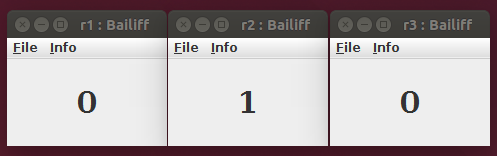
\includegraphics[scale=0.4]{010}
	\caption{Player1 joins. No reason to do anything.}
	\label{fig010}
\end{figure}

\begin{figure}[h!]
	\centering
	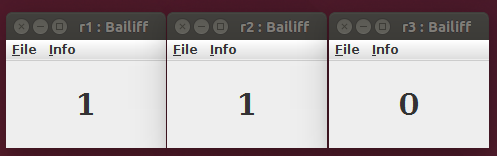
\includegraphics[scale=0.4]{110}
	\caption{Player2 joins. Still no reason to move.}
	\label{fig110}
\end{figure}

\begin{figure}[h!]
	\centering
	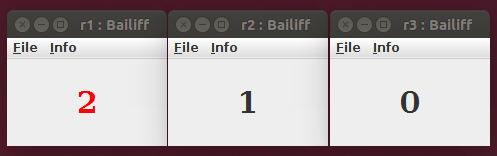
\includegraphics[scale=0.4]{210.png}
	\caption{Player3 (it) joins the same bailiff as Player2. Player3 will try to tag Player2, and Player2 will try to run to the empty bailiff.}
	\label{fig210}
\end{figure}

\begin{figure}[h!]
	\centering
	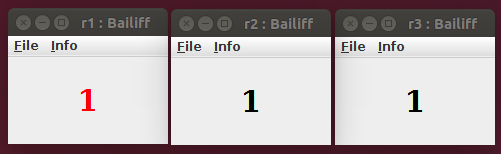
\includegraphics[scale=0.4]{111}
	\caption{Player3 managed to tag Player2 and ran away, or Player2 managed to run away. In either case "it" is now alone in Bailiff 1.}
	\label{fig111}
\end{figure}

\end{document}


